\documentclass[11pt]{article} 

\usepackage[utf8]{inputenc} 

\usepackage{graphicx}

\usepackage{geometry}


\geometry{a4paper} 


\title{Winterthur Yard: Abschlussbericht Projekt}
\author{Maja Fritschi, Raphael Spörri, Florian Bosshard}
\date{} 
\begin{document}
\maketitle

\tableofcontents
\newpage

\section{Projektteam}
Das Projekt wird von folgenden Personen entwickelt:
\begin{itemize}
\item Maja Fritschi (fritsmaj)
\item Raphael Spörri (sporrra0)
\item Florian Bosshard (bosshflo)
\end{itemize}


\section{Umgesetzte Funktionalitäten}
Folgend werden Funktionalitäten aufgelistet die bis zum18. Dezember 2013 umgesetzt wurden: 
\begin{itemize}
\item Der Spieler kann sich auf der Startseite mit einem Usernamen einloggen. Geprüft wird nur, ob er etwas eingibt. Kein Username ist nicht erlaubt. Ausserdem kann man auch nicht auf eine Subseite zugreiffen, wenn man sich nicht eingeloggt hat.
\item Hat der Spieler sich erfolgreich eingeloggt, sieht er einen  Kartenausschnitt der Winterthureraltstatt. Weiter wird ihm mit einem roten Icon angezeigt, wo er sich befindet. Andere Spieler die ebenfalls angemeldet sind werden mit einem blauen Icons angezeigt. Der MisterX wird zu beginn noch nicht angezeigt.
\item Befindet sich der Spieler auf einem der eingezeichneten Koordinaten-Punkte, kann er den Button ``MisterX fangen'' drücken. Es wird ihm im Erfolgsfall gesagt, dass er den MisterX gefangen hat.  Ansonsten erfährt er wo sich der MisterX zu einem bestimmten Zeitpunkt befunden hat. Der ehemalige Standpunkt vom MisterX wird nun auch auf der Karte eingezeichnet. 
\item Wählt man einen auf der Karte eingezeichneten Mitspiele, erfährt man, wie er heisst und wann er sich an diesem Standort befunden hat.
\end{itemize}

Die aktuelle Applikation kann unter http://yard.prusik.ch angeschaut werden. 

\section{Technologien}
\begin{itemize}
\item Für die Karte wurde Open Street Map (http://www.openstreetmap.ch) verwendet. Dies ist eine freie Wiki World Map.
\item Für die Kommunikation via Rest wurde das SLIM-Framework (http://http://www.slimframework.com) verwendet. Dieses Framwork hilft auf eine einfache Weise eine Rest-Schnittstelle zu erstellen. In der Abbildung sieht man den Aufbau im Php-File.
\end{itemize}
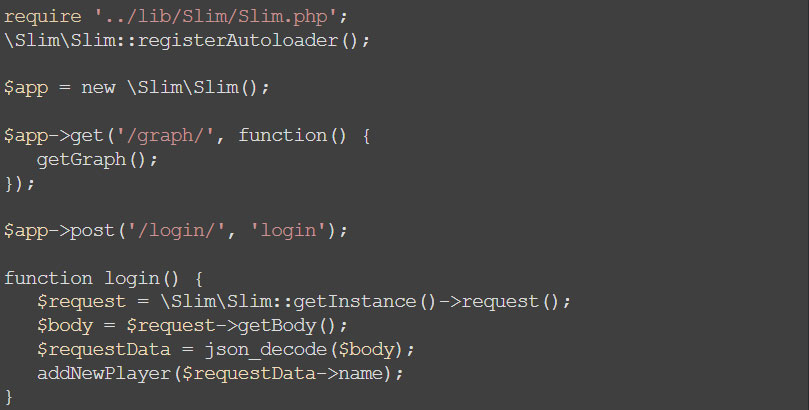
\includegraphics[width=14cm]{Bilder/slim.jpg}

\begin{itemize}
\item Der Aufruf erfolgt wie unten gezeigt via JQuery.
\end{itemize}
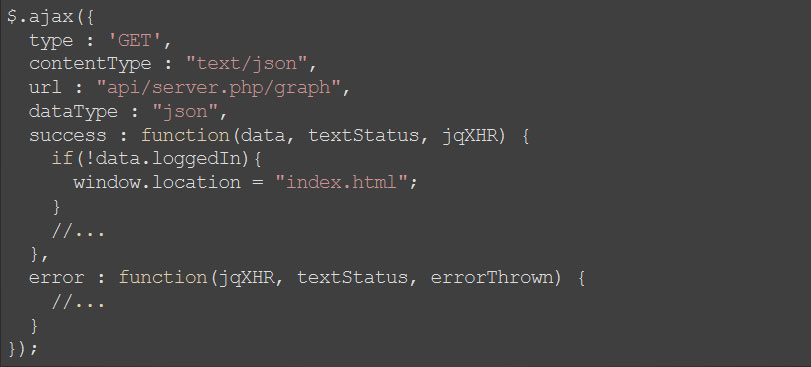
\includegraphics[width=14cm]{Bilder/jquery.jpg}




\section{Abschliessend}
Es hat sehr viel Spass gemacht die App zu erstellen und sie könnte noch an vielen Stellen erweitert werden. Da die Grundfunktionen jetzt implementiert sind, kann sie aber für dieses Projekt als abgeschlossen betrachtet werden. 
Wir wünschen viel Spass beim ausprobieren.





\end{document}
